% ****** Start of file apssamp.tex ******
%
%   This file is part of the APS files in the REVTeX 4.1 distribution.
%   Version 4.1r of REVTeX, August 2010
%
%   Copyright (c) 2009, 2010 The American Physical Society.
%
%   See the REVTeX 4 README file for restrictions and more information.
%
% TeX'ing this file requires that you have AMS-LaTeX 2.0 installed
% as well as the rest of the prerequisites for REVTeX 4.1
%
% See the REVTeX 4 README file
% It also requires running BibTeX. The commands are as follows:
%
%  1)  latex apssamp.tex
%  2)  bibtex apssamp
%  3)  latex apssamp.tex
%  4)  latex apssamp.tex
%
\documentclass[%
 reprint,
%superscriptaddress,
%groupedaddress,
%unsortedaddress,
%runinaddress,
%frontmatterverbose, 
%preprint,
%showpacs,preprintnumbers,
%nofootinbib,
%nobibnotes,
%bibnotes,
 amsmath,amssymb,
 aps,
%pra,
%prb,
%rmp,
%prstab,
%prstper,
%floatfix,
]{revtex4-1}

\usepackage{graphicx}% Include figure files
\usepackage{dcolumn}% Align table columns on decimal point
\usepackage{bm}% bold math
%\usepackage{hyperref}% add hypertext capabilities
%\usepackage[mathlines]{lineno}% Enable numbering of text and display math
%\linenumbers\relax % Commence numbering lines

%\usepackage[showframe,%Uncomment any one of the following lines to test 
%%scale=0.7, marginratio={1:1, 2:3}, ignoreall,% default settings
%%text={7in,10in},centering,
%%margin=1.5in,
%%total={6.5in,8.75in}, top=1.2in, left=0.9in, includefoot,
%%height=10in,a5paper,hmargin={3cm,0.8in},
%]{geometry}

\begin{document}

\title{Effects of pulsed hollow electron lens operation on the beam core in HL-LHC: \\First experimental studies and simulations.}% Force line breaks with \\
\thanks{Fermilab is operated by Fermi Research Alliance, LLC under
	Contract No.~DE-AC02-07CH11359 with the United States Department of
	Energy. This work was partially supported by the US DOE LHC
	Accelerator Research Program (LARP) and by the European FP7 HiLumi
	LHC Design Study, Grant Agreement 284404.}

\author{Miriam Fitterer}
 \email{mfittere@fnal.gov}
\author{Giulio Stancari}%
\author{Alexander Valishev}%
\affiliation{Fermi National Accelerator Laboratory, Batavia, Illinois, USA
% This line break forced with \textbackslash\textbackslash
}%

\author{Giulia Papotti}
\author{Stefano Redaelli}
\author{Daniel Valuch}
\affiliation{CERN, Geneva, Switzerland}%

\date{\today}% It is always \today, today,
             %  but any date may be explicitly specified

\begin{abstract}
In the HL-LHC a considerable amount of energy is stored in the beam tails due to the high beam intensity and an overpopulation of the tails compared to a Gaussian distribution. To control and clean the tail population, the installation of two hollow electron lenses, one per beam, is considered. Beside the DC operation, also a pulsed operation of the hollow electron lens is considered, which would considerably increase the diffusion speed by putting noise on the halo particles. In the ideal case, that is in case of no field at the beam core, only the halo particles are excited while leaving the core unperturbed. The picture though changes, if a residual field is present also at the location of the beam core putting noise also on the beam core. In this paper we present for estimates of the residual field at the beam core expected from the HL-LHC hollow electron lens and first experimental results of the effect of this excitation on the beam core together with the supporting simulations.
\end{abstract}

% PACS 2008:
% 29.20.db Storage rings and colliders

\pacs{29.20.D-}% PACS, the Physics and Astrtheonomy
                             % Classification Scheme.
%\keywords{Suggested keywords}%Use showkeys class option if keyword
                              %display desired
\maketitle

%\tableofcontents

\section{\label{sec:intro}Introduction}%force line break with \protect\\
Looking back and forward at the last, current and future high energy and intensity accelerators, each new machine represents a considerable leap in stored beam energy with rising values for future accelerators and Colliders (see Table~\ref{tab:stored_energy})
\begin{table*}%The best place to locate the table environment is directly after its first reference in text
	\caption{\label{tab:stored_energy}%
		Stored beam energy for different past, present and future colliders. Each new machine represents a leap in stored beam energy.
	}
	\begin{ruledtabular}
		\begin{tabular}{lccccc}
			Collider& Tevatron (protons) \cite{tevatron} & LHC 2016 & LHC nominal & HL-LHC & FCC\\
			\colrule
			Beam energy [GeV] & 980 & ? & ? & ? & \\
			Number of bunches & 36 & ? & ? & ? & \\
			Number of particles per bunch & $2.9\times 10^{11}$ & ? & ? & ? & \\
			Stored beam energy [MJ] & 1.6 & ? & ? & ? & \\
		\end{tabular}
	\end{ruledtabular}
\end{table*}

- why do we need active halo control -> refer to different methods -> say that e-lens is superior as shown in review
- layout
\begin{figure}[h]
	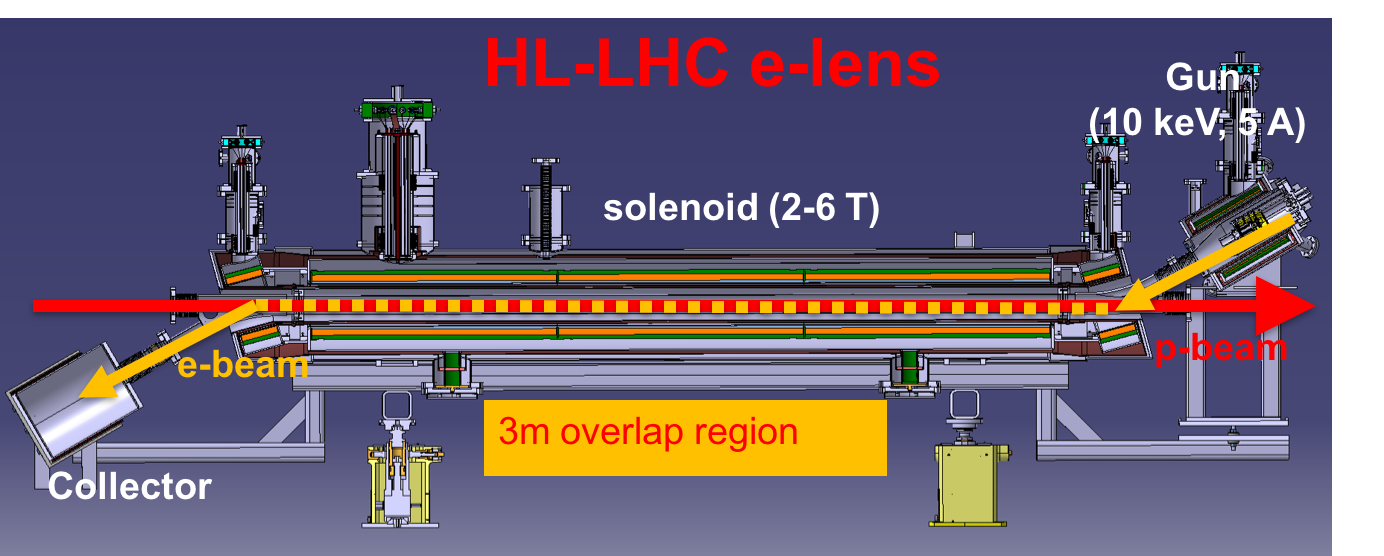
\includegraphics[width=1.0\linewidth]{hel_layout}% Here is how to import EPS art
	\caption{\label{fig:hel_layout} Layout of HEL \textbf{Ask Diego how to acknowledge correctly}.}
\end{figure}



\begin{acknowledgments}
We wish to acknowledge the support of the author community in using
REV\TeX{}, offering suggestions and encouragement, testing new versions,
\dots.
\end{acknowledgments}

\appendix

\section{Appendixes}


\bibliography{bibliography}% Produces the bibliography via BibTeX.

\end{document}
%
% ****** End of file apssamp.tex ******
